% Desenvolvimento
O principal método de otimização desenvolvido a fim de solucionar os problemas de programação quadrática é o método de Newton que busca uma aproximação de segunda ordem da função objetivo por meio da série de Taylor. Este método, considerando funções perfeitamente quadrática, possui convergência rápida. Todavia, devido a necessidade de determinar a derivada de primeira e de segunda ordem da função objetivo, o seu esforço computacional pode ser elevado. Além disso, em muitos casos os problemas são considerados uma caixa preta, ou seja, a função objetivo não está disponível; e em outros casos, mesmo a função objetivo estando disponível, o cálculo de suas derivadas de primeira e de segunda ordem é uma operação extremamente complexa. Isso implica na utilização de métodos numéricos para a determinação das derivadas, acarretando em um custo computacional ainda mais elevado.
Todo esse cenário proporcionou o desenvolvimento de novos métodos de otimização, que buscam manter a qualidade de convergência do método de Newton e, simultaneamente, diminuir o custo computacional por meio de calcular as derivadas da função objetivo de forma aproximada. Como já abordado nesse trabalho, esses métodos são conhecidos como métodos Quase-Newton.
A fim de verificar e comparar o desempenho dos algoritmos da família de métodos Quase-Newton (o BFGS e o DFP nas suas formas tradicionais e com as adaptações de Huang e de Biggs) serão consideradas seis funções de teste, as quais são apresentadas nas próximas seções.

\subsection{Primeira Função de Teste}

A primeira função de teste se trata de uma função objetivo com variável de decisão e de dimensão dada por:

\begin{equation}\label{eq:prifuntst}
  f(x)= \frac{1}{2}*(x-c)^{T}*A*(x-c)
\end{equation}

Onde $c$ é um vetor unitário e $A$ é uma matriz diagonal. Ressalta-se que para os casos estudados é a matriz identidade. Esses parâmetros são apresentados abaixo:

\begin{equation*}
    X_{1xn} = \begin{bmatrix}
                    X_1 & X_2 & \ldots & X_n
                \end{bmatrix}    
\end{equation*}
\begin{equation*}
    C_{1xn} = \begin{bmatrix}
                    1 & 1 & \ldots & 1
                \end{bmatrix}    
\end{equation*}
\begin{equation*}
    A_{nxn} = \begin{bmatrix}
                    1 & 0 & \ldots & 0 & 0 \\
                    0 & 1 & \ldots & 0 & 0 \\
                    \vdots & \vdots & \ddots & \vdots & \vdots \\
                    0 & 0 & \ldots & 1 & 0 \\
                    0 & 0 & \ldots & 0 & 1 \\
                \end{bmatrix}    
\end{equation*}

O gradiente da função apresentada em \ref{eq:prifuntst} é dado por:

\begin{equation}\label{eq:gradprifuntst}
    \nabla f(x) = A*(x-c)
\end{equation}

Os gráficos dessa função, do gradiente e das curvas de nível considerando duas variáveis são ilustrados abaixo:

\begin{figure}[h!]
    \centering 
    \subfloat[][Função objetivo]{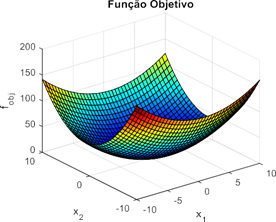
\includegraphics[scale=1]{img/section2/prifun.png}\label{<figure1>}}    
    \qquad
    \subfloat[][Gradiente da função objetivo]{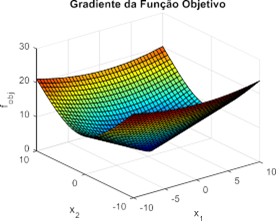
\includegraphics[scale=1]{img/section2/graprifun.png}\label{<figure2>}} 
    \qquad
    \subfloat[][Curvas de nível]{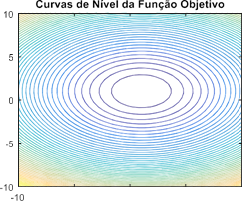
\includegraphics[scale=1]{img/section2/nivelprifun.png}\label{<figure2>}} 
    \caption{Primeira função de teste}%
    \label{fig:fig1}%
\end{figure}
 \FloatBarrier
Ao observar os gráficos ilustrados nas figuras 1 e 2 é fácil notar que a função apresentada em \ref{eq:prifuntst} é uma função quadrática deslocada com o mínimo posicionado em $X_{1xn}=[\ 1 , 1 , \ldots , 1 ]\ $ (em duas dimensões um paraboloide).

\subsection{Segunda Função de Teste}

A segunda função de teste se trata de uma função objetivo com duas variáveis independentes com termos quadráticos e um cúbico, em que o termo cúbico deve apresentar menor influência no caso de se utilizar métodos Quase-Newton para determinar o mínimo da função. Essa função é definida como apresentado abaixo:

\begin{equation}\label{eq:secfuntst}
  f(x) = 12*x_1^2 - 4*x_2^2 - 12*x_1x_2 + 2*x_1 + a*(x_1^3+x_2^3)
\end{equation}

onde $a$ é um parâmetro que assume valores que ponderam a influência do termo cúbico na função. O gradiente da função apresentada em \ref{eq:secfuntst} pode ser escrito como se segue:

\begin{equation}\label{eq:gradsecfuntst}
    \nabla f(x) = \begin{cases}
        24*x_1-12*x_2+2+3*a*x_1^2\\
       8*x_2-12*x_1+3*a*x_2^2
    \end{cases}
\end{equation}

A solução ótima desse problema pode ser determinada ao considerar $\nabla f(x)=0$. Nesse caso, conforme pode ser observado pelo sistema de equações em \ref{eq:gradsecfuntst}, a solução ótima é dependente da escolha de $a$ , podendo ser obtida por meio da resolução desse sistema.
Os gráficos da função em \ref{eq:secfuntst}, do gradiente e das curvas de nível considerando valores do parâmetro $a$ igual a zero e igual a um são ilustrados abaixo:


\subsection{Terceira Função de Teste}
\subsection{Quarta Função de Teste}
\subsection{Quinta Função de Teste}
\subsection{Sexta Função de Teste}

\subsection{Considerações dos Experimentos}
  A Tabela \ref{tab:tab_doe} apresenta de forma sumarizada como os experimentos devem ser realizados e analisados.
  % Please add the following required packages to your document preamble:
% \usepackage{multirow}
% \usepackage{graphicx}
% \usepackage[table,xcdraw]{xcolor}
% If you use beamer only pass "xcolor=table" option, i.e. \documentclass[xcolor=table]{beamer}
\begin{table}[h!]
\resizebox{\textwidth}{!}{%
\begin{tabular}{c|cccccc|}
\cline{2-7}
 &
 \multicolumn{6}{c|}{\cellcolor[HTML]{EFEFEF}Experimentos} \\ \cline{2-7} 
\multirow{-2}{*}{} &
 \multicolumn{1}{c|}{\cellcolor[HTML]{EFEFEF}1º} &
 \multicolumn{1}{c|}{\cellcolor[HTML]{EFEFEF}2º} &
 \multicolumn{1}{c|}{\cellcolor[HTML]{EFEFEF}3º} &
 \multicolumn{1}{c|}{\cellcolor[HTML]{EFEFEF}4º} &
 \multicolumn{1}{c|}{\cellcolor[HTML]{EFEFEF}5º} &
 \cellcolor[HTML]{EFEFEF}6º \\ \hline
\multicolumn{1}{|c|}{\cellcolor[HTML]{EFEFEF}Descrissão} &
 \multicolumn{1}{c|}{\begin{tabular}[c]{@{}c@{}}Avaliação das \\ Funções \\ quadráticas\end{tabular}} &
 \multicolumn{1}{c|}{\begin{tabular}[c]{@{}c@{}}Avaliação das \\ funções não \\ quadráticas\end{tabular}} &
 \multicolumn{1}{c|}{\begin{tabular}[c]{@{}c@{}}Avaliação do \\ custo \\ computacional \\ em função da \\ variação da \\ dimensão\end{tabular}} &
 \multicolumn{1}{c|}{\begin{tabular}[c]{@{}c@{}}Técnica da Seção \\ Áurea Avaliação \\ direta da função e \\ aproximações \\ quadráticas da \\ função a cada \\ iteração\end{tabular}} &
 \multicolumn{1}{c|}{\begin{tabular}[c]{@{}c@{}}Avaliação dos \\ métodos Quase- \\ Newton em \\ problemas com \\ Hessiana singular\end{tabular}} &
 \begin{tabular}[c]{@{}c@{}}Avaliação \\ estatística \\ dos métodos \\ Quase \\ Newton com \\ a variação do \\ \textbf{Parâmetro} $\alpha$\end{tabular} \\ \hline
\multicolumn{1}{|c|}{\cellcolor[HTML]{EFEFEF}} &
 \multicolumn{1}{c|}{1ª Função de Teste} &
 \multicolumn{1}{c|}{} &
 \multicolumn{1}{c|}{} &
 \multicolumn{1}{c|}{4ª Função de Teste} &
 \multicolumn{1}{c|}{} &
  \\
\multicolumn{1}{|c|}{\cellcolor[HTML]{EFEFEF}} &
 \multicolumn{1}{c|}{2ª Função de Teste} &
 \multicolumn{1}{c|}{} &
 \multicolumn{1}{c|}{} &
 \multicolumn{1}{c|}{5º Função de Teste} &
 \multicolumn{1}{c|}{} &
  \\
\multicolumn{1}{|c|}{\multirow{-3}{*}{\cellcolor[HTML]{EFEFEF}\begin{tabular}[c]{@{}c@{}}Funções \\ Avaliadas\end{tabular}}} &
 \multicolumn{1}{c|}{3ª Função de Teste} &
 \multicolumn{1}{c|}{\multirow{-3}{*}{2ª Função de Teste}} &
 \multicolumn{1}{c|}{\multirow{-3}{*}{4ª Função de Teste}} &
 \multicolumn{1}{c|}{} &
 \multicolumn{1}{c|}{\multirow{-3}{*}{6º Função de Teste}} &
 \multirow{-3}{*}{2ª Função de Teste} \\ \hline
\multicolumn{1}{|c|}{\cellcolor[HTML]{EFEFEF}} &
 \multicolumn{1}{c|}{fex1} &
 \multicolumn{1}{c|}{} &
 \multicolumn{1}{c|}{} &
 \multicolumn{1}{c|}{fexLivro} &
 \multicolumn{1}{c|}{} &
  \\
\multicolumn{1}{|c|}{\cellcolor[HTML]{EFEFEF}} &
 \multicolumn{1}{c|}{fexLivro} &
 \multicolumn{1}{c|}{} &
 \multicolumn{1}{c|}{} &
 \multicolumn{1}{c|}{fex1} &
 \multicolumn{1}{c|}{} &
  \\
\multicolumn{1}{|c|}{\multirow{-3}{*}{\cellcolor[HTML]{EFEFEF}\begin{tabular}[c]{@{}c@{}}Código das \\ Funções Avaliadas \\ no Matlab\end{tabular}}} &
 \multicolumn{1}{c|}{fex3} &
 \multicolumn{1}{c|}{\multirow{-3}{*}{fexLivro}} &
 \multicolumn{1}{c|}{\multirow{-3}{*}{fex1}} &
 \multicolumn{1}{c|}{fun\_rosensuzuki\_irr} &
 \multicolumn{1}{c|}{\multirow{-3}{*}{f\_tiltednormcond}} &
 \multirow{-3}{*}{fexLivro} \\ \hline
\end{tabular}%
}
\caption{Detalhamento dos experimentos realizados para as análises dos Métodos Quase-Newton.}
\label{tab:tab_doe}
\end{table}

Nos experimentos realizados nesse trabalho alguns Parâmetros devem ser fixados a fim executar os algoritmos desenvolvidos em ambiente Matlab e possibilitar uma análise adequada. A descrição de tais Parâmetros de uma forma geral e mais especifica, considerando os experimentos, é apresentada abaixo:
\begin{itemize}
  \item \textbf{Parâmetro}: $Imetqn\rightarrow$ Chaveia o algoritmo Quase-Newton a ser executado
  \item \textbf{Parâmetro}: $icaso\rightarrow$ Chaveia a função objetivo a ser estudada
  \item \textbf{Parâmetro}: $a\rightarrow$ Pondera os termos não quadráticos
  \item \textbf{Parâmetro}: $dim\rightarrow$ Determina a dimensão do problema a ser resolvido
  \item \textbf{Parâmetro}: $xstar\rightarrow$ Estabelece a solução ótima do problema
  \item \textbf{Parâmetro}: $x0\rightarrow$ Estabelece o ponto inicial
  \item \textbf{Parâmetro}: $isa\_FV\rightarrow$ Chaveia a técnica da Seção Áurea
\end{itemize}

A função desenvolvida no Matlab que soluciona os problemas propostos nesse trabalho é codificada como \textbf{otqnmat\_a77}. Os parâmetros dessa função são pontuados a seguir:

\begin{itemize}
  \item \textbf{Parâmetro de entrada}: $funcao\rightarrow$ Função a ser aproximada
  \item \textbf{Parâmetro de entrada}: $isa\_FV\rightarrow$ Seção Áurea
  \item \textbf{Parâmetro de entrada}: $Imetqn\rightarrow$ Método Quase-Newton escolhido 
  \item \textbf{Parâmetro de entrada}: $MAXITER\rightarrow$ Número máximo de iterações 
  \item \textbf{Parâmetro de entrada}: $x0\rightarrow$ Ponto inicial
  \item \textbf{Parâmetro de entrada}: $xMin\rightarrow$ Limite inferior 
  \item \textbf{Parâmetro de entrada}: $xMAx\rightarrow$ Limite superior 
  \item \textbf{Parâmetro de entrada}: $epslon\rightarrow$ Precisão
  \item \textbf{Parâmetro de saída}: $XK1\rightarrow$ Armazena a solução das variáveis de decisão 
  \item \textbf{Parâmetro de saída}: $Hfobjrightarrow$ Armazena os valores da função objetivo 
  \item \textbf{Parâmetro de saída}: $icfunc\rightarrow$ Número de avaliações da função objetivo
\end{itemize}

Finalmente, a precisão que define um dos critérios de parada dos algoritmos Quase-Newton executados nesse trabalho será $10^{-6}$ . Sendo \textbf{dim} a dimensão do problema de otimização a ser resolvido. O número máximo de iterações define um segundo critério de parada e será:

\[ \textrm{N\degree Máximo de Iteração} = 2 * dim * 100\]